%==============================================================
%  SLIDE BAO VE -- BAO CAO GIAI TICH SO
%  Bien dich: latexmk -xelatex slide.tex   (bat buoc XeLaTeX)
%==============================================================
\documentclass[aspectratio=169,11pt]{beamer}

\usetheme{metropolis}
\metroset{block=fill, numbering=fraction, progressbar=frametitle}

%--------------------- FONT & TIENG VIET ---------------------
\usepackage{fontspec}
\usepackage{polyglossia}
\setdefaultlanguage{vietnamese}
\setotherlanguage{english}
\setmainfont{TeX Gyre Heros}
\setsansfont{TeX Gyre Heros}
\setmonofont{DejaVu Sans Mono}[Scale=0.82]

\usepackage{amsmath,amssymb,bm}
\usepackage{booktabs}
\usepackage{multirow}
\usepackage{animate}   % animation nhung trong PDF (Adobe Reader, Okular, Foxit)

% Animation lay tu anim/<ten>.pdf -- moi trang mot khung, sinh boi
% code/pinns/animate.py. Trong trinh xem khong ho tro, hien khung dau.
\newcommand{\hoathinh}[2][0.62\textheight]{%
  \animategraphics[height=#1,controls=play,loop,autoplay]{10}{anim/#2}{}{}}

%--------------------- KY HIEU DUNG CHUNG ---------------------
\newcommand{\R}{\mathbb{R}}
\newcommand{\bx}{\bm{x}}
\newcommand{\bk}{\bm{k}}
\newcommand{\bW}{\bm{W}}
\newcommand{\btheta}{\bm{\theta}}
\newcommand{\Net}{\mathrm{Net}}
\newcommand{\Lop}{\mathcal{L}}
\newcommand{\norm}[1]{\left\lVert #1 \right\rVert}
\newcommand{\abs}[1]{\left\lvert #1 \right\rvert}

% mau nhan manh
\definecolor{good}{RGB}{20,120,70}
\definecolor{bad}{RGB}{170,40,40}
\newcommand{\good}[1]{\textcolor{good}{\textbf{#1}}}
\newcommand{\bad}[1]{\textcolor{bad}{\textbf{#1}}}

%--------------------- SIEU DU LIEU ---------------------
% Tieu de bao cao dai hai dong, khung title mac dinh cua metropolis khong
% du cao. Thu nho co chu tieu de va nen khoang cach thay vi cat tieu de.
\setbeamerfont{title}{size=\large, series=\bfseries}
\setbeamerfont{subtitle}{size=\small}
\setbeamerfont{author}{size=\small}
\setbeamerfont{institute}{size=\footnotesize}
\setbeamerfont{date}{size=\footnotesize}
\title{Cơ sở lý thuyết về mạng nơ-ron\\ và phương pháp PINNs cho phương trình vi phân}
\subtitle{Báo cáo Giải tích số}
\author{Nguyễn Hoàng Tú \quad\textbar\quad MSSV 23110220}
\institute{Khoa Toán--Tin học, ĐH Khoa học Tự nhiên, ĐHQG-HCM\\
  GVHD: TS.\ Ông Thanh Hải}
\date{Tháng 9 năm 2026}

\begin{document}

\maketitle

%==============================================================
\begin{frame}{Hai câu hỏi của báo cáo}
\small
PINNs thay không gian hàm thử của phần tử hữu hạn bằng một \alert{mạng nơ-ron}:
cực tiểu hoá phần dư $r_{\btheta} = \Lop[u_{\btheta}] - f$ tại các điểm phối trí.

\medskip
\begin{columns}[T]
\begin{column}{0.47\textwidth}
\begin{block}{Câu hỏi 1}
Vì sao cực tiểu hoá \emph{phần dư} lại là việc đáng làm?

\smallskip
\footnotesize Phần dư \emph{tính được}; sai số mới là thứ ta \emph{quan tâm}.
\end{block}
\end{column}
\begin{column}{0.47\textwidth}
\begin{block}{Câu hỏi 2}
Vì sao phương pháp hỏng trên bài toán có thang độ dài nhỏ?

\smallskip
\footnotesize Burgers với $\nu = 0{,}01/\pi$ là ví dụ chuẩn mực.
\end{block}
\end{column}
\end{columns}

\medskip
\centering
\alert{Trả lời cả hai, rồi kiểm chứng bằng chín thí nghiệm.}
\end{frame}

%==============================================================
\begin{frame}{Trọng tâm khác với tài liệu học sâu thông thường}
Tài liệu học sâu khảo sát đạo hàm theo \emph{tham số} $\btheta$.
PINNs cần đạo hàm theo \alert{biến đầu vào} $\bx$.

\medskip
\begin{block}{Hai hệ thức truy hồi (Mệnh đề 2.6, 2.7)}
\vspace{-2mm}
\[
\bm{G}^{(\ell)} = \bm{D}^{(\ell)}\bW^{(\ell)}\bm{G}^{(\ell-1)},
\qquad
\bm{S}^{(\ell)}_k
 = \underbrace{\sigma''(z^{(\ell)}_k)\,(\bm{g}^{(\ell)}_k)^{\!\top}\bm{g}^{(\ell)}_k}
   _{\text{độ cong \emph{sinh} tại lớp }\ell}
 + \underbrace{\sigma'(z^{(\ell)}_k)\textstyle\sum_j w^{(\ell)}_{kj}\bm{S}^{(\ell-1)}_j}
   _{\text{độ cong \emph{truyền} từ dưới}}
\]
\end{block}

\medskip
Từ đây suy ra ngay một \alert{điều kiện cần} trên hàm kích hoạt:
nếu $\sigma'' \equiv 0$ thì số hạng thứ nhất triệt tiêu ở \emph{mọi} lớp,
và quy nạp cho $\nabla^2_{\bx}\Net_{\btheta} \equiv \bm{0}$.
\end{frame}

%==============================================================
\begin{frame}{Hệ quả sắc nhất: ReLU không "kém", mà \emph{đứng yên}}
\begin{alertblock}{Hệ quả 2.28}
Với $\sigma = \mathrm{ReLU}$ và phương trình bậc hai, hàm mục tiêu phần dư là
\alert{hằng số địa phương}:
\[
J(\btheta') = \tfrac{1}{N_r}\textstyle\sum_i f(x_i)^2
\quad \forall\,\btheta' \in U,
\qquad\text{nên}\qquad \nabla_{\btheta}J(\btheta) = \bm{0}.
\]
\end{alertblock}

\medskip
Mạnh hơn hẳn cách nói thông thường "ReLU cho kết quả kém": mọi thuật toán gradient
đứng yên \alert{tuyệt đối} --- không phải học chậm, mà không học gì cả.

\medskip
\begin{block}{Đo được (Thí nghiệm 1)}
$\norm{\nabla J_r}_\infty = \good{0{,}0}$ đúng nghĩa;
$J_r = 776{,}23$ so với giá trị lý thuyết $778{,}49$.

\smallskip
\footnotesize Điều kiện $\sigma \in C^m$ là \emph{bắt buộc}, không phải khuyến nghị.
\end{block}
\end{frame}

%==============================================================
\begin{frame}{Xem nó xảy ra: ReLU đứng yên, tanh hội tụ}
\centering
\hoathinh{tn1_relu_vs_tanh}

\medskip
\footnotesize Đường cam nằm yên ở $J_r = 776{,}23$ suốt $4\,000$ vòng ---
đúng giá trị Hệ quả 2.28 tiên đoán. \textcolor{gray}{(Animation phát trong
Adobe Reader / Okular.)}
\end{frame}

%==============================================================
\begin{frame}{Câu hỏi 1: vì sao cực tiểu hoá phần dư là đáng làm}
\begin{block}{Chặn ổn định (Mệnh đề 4.3) --- bài toán Poisson một chiều}
Nếu $u_{\btheta}$ thoả điều kiện biên \emph{chính xác}:
\[
\norm{e_{\btheta}}_{L^2} \;\le\; \frac{1}{\pi^{2}}\,\norm{r_{\btheta}}_{L^2}
\]
\end{block}

Mắt xích biện minh cho toàn bộ phương pháp: phần dư nhỏ \emph{khống chế được} sai số.

\medskip
\begin{alertblock}{Nhưng hằng số suy biến (Mệnh đề 4.4)}
Với $-\nu u'' + u' = f$:
$\quad\norm{e_{\btheta}}_{L^2} \le \dfrac{1}{\pi^{2}\nu}\,\norm{r_{\btheta}}_{L^2}$

\smallskip
Khi $\nu$ nhỏ, \bad{phần dư nhỏ không còn bảo đảm sai số nhỏ.}
\end{alertblock}
\end{frame}

%==============================================================
\begin{frame}{Câu hỏi 2: ba nguyên nhân ở ba tầng khác nhau}
\small
\begin{table}
\small
\begin{tabular}{@{}lp{7.6cm}@{}}
\toprule
\textbf{Tầng} & \textbf{Cơ chế} \\
\midrule
Bài toán vi phân & hằng số ổn định tỉ lệ $1/\nu$ \\[2pt]
Tối ưu & toán tử vi phân khuếch đại tần số cao theo $\norm{\bk}^m$,
  làm phổ Hessian trải rộng \\[2pt]
Xấp xỉ & biểu diễn tần số $\bk$ đòi hỏi chuẩn tham số cỡ $\norm{\bk}^{d+1}$,
  ngược chiều với khởi tạo \\
\bottomrule
\end{tabular}
\end{table}

\medskip
\begin{alertblock}{Hệ quả phương pháp luận}
Vì ba nguyên nhân nằm ở ba tầng khác nhau,
\alert{không kỹ thuật nào tác động lên một tầng có thể sửa được hai tầng còn lại.}
Cân bằng trọng số chỉ chạm tầng giữa; nó không cứu được bài toán mà hằng số
ổn định đã suy biến.
\end{alertblock}
\end{frame}

%==============================================================
\begin{frame}{Thiết kế thực nghiệm}
\begin{columns}[T]
\begin{column}{0.5\textwidth}
\textbf{Nguyên tắc}
\begin{itemize}
\item PyTorch thuần, \emph{không} dùng thư viện PINNs đóng gói
\item Mỗi thí nghiệm trả lời một câu hỏi cụ thể
\item Tiêu chí thành/bại xác định \alert{trước} khi chạy
\item Mã nguồn công bố kèm báo cáo
\end{itemize}
\end{column}
\begin{column}{0.47\textwidth}
\textbf{Mười thí nghiệm}
\begin{itemize}\footnotesize
\item[TN1] hàm kích hoạt, ReLU
\item[TN2] cái giá của ràng buộc mềm
\item[TN3] thiên kiến phổ
\item[TN4] khuếch tán (đối chứng lành mạnh)
\item[TN5] Burgers (bài toán cứng)
\item[TN6] kiểm chứng chặn ổn định
\item[TN7] quét $\nu$
\item[TN8] độ phân tán giữa hạt giống
\item[TN9] chi phí tính toán
\item[TN10] \alert{Burgers, áp dụng chính các biện pháp khắc phục}
\end{itemize}
\end{column}
\end{columns}
\end{frame}

%==============================================================
\begin{frame}{TN3: thiên kiến phổ bị \emph{đảo chiều}}
Nghiệm chế tạo đa tần số, biên độ \emph{bằng nhau}:
$u^{\star}(x) = \sum_{k\in\{1,4,8\}}\sin(2\pi k x)$.

\medskip
\begin{columns}[T]
\begin{column}{0.48\textwidth}
\begin{block}{Hồi quy ($P \equiv 1$)}
Học tần số \good{thấp trước}: $t_{10}$ tăng đơn điệu theo $k$ ở \good{5/5} hạt giống,
ba khoảng tách bạch hoàn toàn.
\end{block}
\end{column}
\begin{column}{0.48\textwidth}
\begin{alertblock}{Phần dư ($P(k) = 4\pi^2k^2$)}
\bad{Ngược lại}: sai số dồn về mode tần số \emph{thấp};
$\abs{c_1}/\abs{c_8} > 1$ ở 5/5 hạt giống.
\end{alertblock}
\end{column}
\end{columns}

\medskip
\begin{block}{Hệ quả: phải sửa chính chương lý thuyết}
Mục 4.3.4 kết luận "bài toán đòi hỏi độ chính xác cao nhất ở đúng những tần số mà
mô hình học chậm nhất". \alert{Không đúng phổ quát} --- với toán tử elliptic thuần
tuý, hàm mục tiêu phần dư \emph{ưu tiên} tần số cao.
\end{block}
\end{frame}

%==============================================================
\begin{frame}{Xem nó xảy ra: thứ tự học bị đảo chiều}
\centering
\hoathinh[0.68\textheight]{tn3_thien_kien_pho}

\footnotesize Hồi quy học $k=1$ trước, $k=8$ sau cùng.
Với hàm mục tiêu phần dư, sai số lại dồn về $k=1$.
\end{frame}

%==============================================================
\begin{frame}{TN4 \& TN5: bệnh lý gradient \emph{phụ thuộc bài toán}}
Chỉ số mất cân bằng $\rho_b$ đo tỉ lệ biên độ gradient giữa các thành phần mất mát.

\medskip
\begin{table}
\small
\begin{tabular}{@{}lll@{}}
\toprule
\textbf{Bài toán} & $\max\rho_b$ (5 hạt giống) & \textbf{Kết luận} \\
\midrule
Khuếch tán, $\nu = 0{,}1$ & $[19{,}5;\ 96{,}5]$   & lành mạnh \\
Burgers, $\nu = 0{,}01/\pi$ & $[603;\ 4\,070]$    & \bad{có bệnh lý} \\
\bottomrule
\end{tabular}
\end{table}

\medskip
\begin{alertblock}{Hai khoảng \emph{không giao nhau}}
Cách biệt ít nhất $6$ lần, trung vị $47$ lần.
Bệnh lý gradient \alert{không phải đặc tính cố hữu của mọi PINN} ---
nên phải \emph{chẩn đoán trước khi can thiệp}.
\end{alertblock}

\footnotesize
Lưu ý: tách biệt về \emph{độ lớn} thì vững; phát biểu về \emph{chiều} biến thiên
chỉ vững ở bài toán cứng (5/5), còn ở bài lành mạnh chỉ 3/5.
\end{frame}

%==============================================================
\begin{frame}{Kết quả tiêu cực sinh ra một kết quả lý thuyết}
\small
Thuật toán ủ trọng số (Wang và cộng sự) được đề xuất đúng cho tình huống này.
Đo được: nó làm sai số \bad{xấu đi ở 10/10 lần chạy}.

\medskip
\begin{alertblock}{Bổ đề 5.11 --- chế độ phản hồi dương}
Quy tắc cập nhật $\hat\lambda_i$ có một vòng phản hồi dương với tốc độ phân kỳ
\[
\hat\lambda_i \;\gtrsim\; J_i^{-1/2}
\]
và \alert{không có cơ chế tự hãm}.
\end{alertblock}

\medskip
Số liệu khớp: $\lambda_b$ chạy tới $10^4$--$10^5$ ở mọi hạt giống, tại đó số hạng
phần dư bị át hoàn toàn.

\centering
\alert{Kết quả lý thuyết nảy sinh \emph{từ} thực nghiệm,
không phải được kiểm chứng bởi nó.}
\end{frame}

%==============================================================
\begin{frame}{TN8: lặp lại mọi thí nghiệm trên năm hạt giống}
\begin{table}
\small
\begin{tabular}{@{}lrl@{}}
\toprule
\textbf{Con số đã trích dẫn} & \textbf{trung vị} & \textbf{khoảng} \\
\midrule
số mũ $-0{,}907$ (TN2)            & $-0{,}64$ & $[-0{,}907;\ -0{,}503]$ \\
tỉ số $38{,}6$ (TN3)              & $5{,}5$   & $[4{,}5;\ 46{,}3]$ \\
cải thiện $161$ lần (TN3)         & $49$      & $[18;\ 83]$ \\
$\varepsilon_{L^2} = 2{,}84\times10^{-2}$ (TN5)
  & $1{,}38\times10^{-1}$ & $[7{,}9\times10^{-3};\ 2{,}1\times10^{-1}]$ \\
\bottomrule
\end{tabular}
\end{table}

\medskip
\begin{alertblock}{Hình mẫu}
\alert{Mọi kết luận định tính đều sống sót 5/5.\\
Không một con số đơn lẻ nào sống sót nguyên vẹn.}
\end{alertblock}

\footnotesize
Ba trong bốn giá trị nằm ở \emph{cực trị hoặc ngoài} dải năm hạt giống ---
khi chạy một lần, ta không có cách nào biết mình đang ở đâu trong dải.
\end{frame}

%==============================================================
\begin{frame}{TN9: chi phí tính toán thực đo}
\small
\begin{table}
\small
\begin{tabular}{@{}lrrr@{}}
\toprule
\textbf{Phương pháp} & $\Delta t$ & \textbf{Thời gian} & $\varepsilon_{L^2}$ \\
\midrule
PINN, $6\,000$ Adam $+$ $800$ L-BFGS & --- & $\approx 170$ s & $1{,}38\times10^{-1}$ \\
Sai phân hữu hạn, $N_x = 63$ & $5\times10^{-3}$ & \good{$0{,}0098$ s} & $7{,}24\times10^{-2}$ \\
\bottomrule
\end{tabular}
\end{table}

\begin{center}
\bad{PINN chậm hơn khoảng $1{,}8\times10^{4}$ lần --- bốn bậc độ lớn.}
\end{center}

\medskip
\begin{block}{Nhưng phải đọc cho đúng phạm vi}
Chương 1 nêu \emph{ba} động lực cho PINNs: bài toán ngược, điều kiện biên khuyết,
lời nguyền số chiều.

\smallskip
\alert{Không động lực nào có mặt} trong lớp bài toán được thực nghiệm: thuận,
đủ dữ liệu, $d = 1$ --- đúng chế độ mà sai phân hữu hạn gần như tối ưu.
\end{block}
\end{frame}

%==============================================================
\begin{frame}{TN10: áp dụng chính các biện pháp báo cáo đề xuất}
\begin{columns}[T]
\begin{column}{0.54\textwidth}
\small
\begin{tabular}{@{}lll@{}}
\toprule
& \textbf{TN5} & \textbf{TN10} \\
\midrule
Mạng & $4\times32$ & $8\times20$ \\
$N_r$ & $2\,500$ & $10\,000$ + RAR \\
L-BFGS & $800$ vòng & $6$ đợt $\times$ $2\,000$ \\
\midrule
$\varepsilon_{L^2}$ trung vị & $1{,}38\times10^{-1}$ & \good{$6{,}48\times10^{-4}$} \\
khoảng, max/min & $26{,}4$ & $2{,}2$ \\
\bottomrule
\end{tabular}

\medskip
\footnotesize Công trình gốc (Raissi 2019): $6{,}7\times10^{-4}$.
\end{column}
\begin{column}{0.43\textwidth}
\begin{block}{Tốt hơn \alert{213 lần}}
Hạt giống \emph{tệ nhất} của TN10 vẫn tốt hơn hạt giống \emph{tốt nhất} của
TN5 gần $10$ lần.
\end{block}
\begin{alertblock}{Nhưng nói cho đúng}
\footnotesize
\begin{itemize}
\item $83\%$ mức cải thiện (thang log) có \emph{trước} điểm RAR đầu tiên;
  tách biến: RAR chỉ góp $\sim 2\%$.
\item Vẫn chậm hơn sai phân hữu hạn $\sim 10^{4}$ lần.
\end{itemize}
\end{alertblock}
\end{column}
\end{columns}
\end{frame}

%==============================================================
\begin{frame}{Tách biến: RAR giúp ở đâu?}
\centering
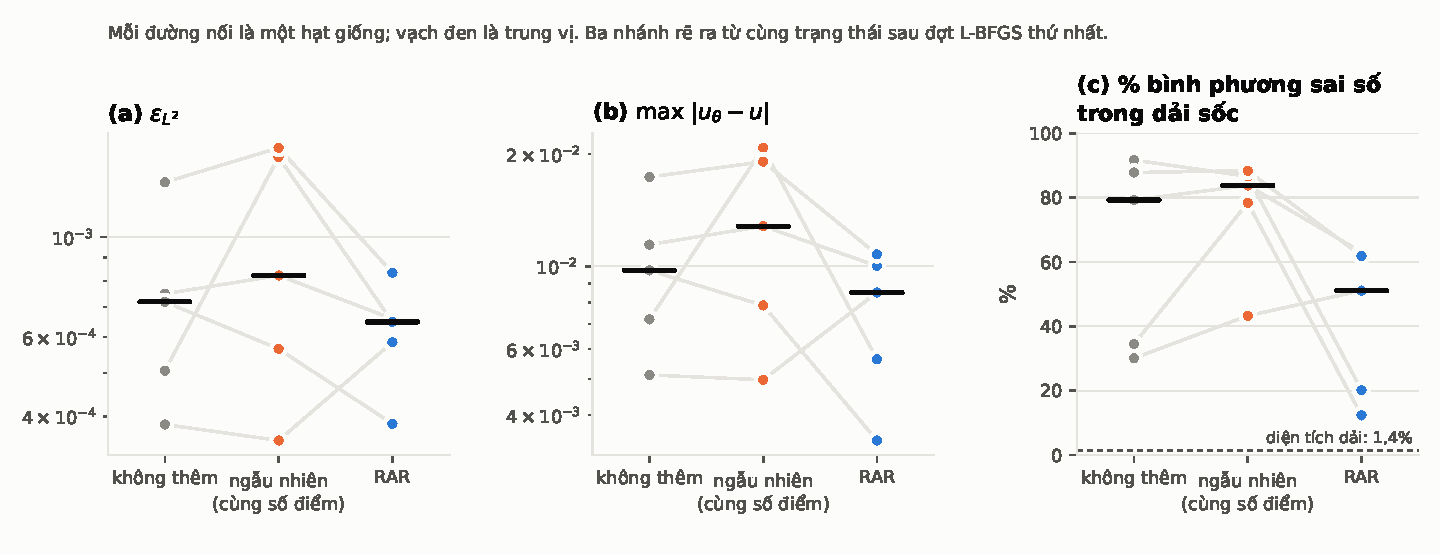
\includegraphics[width=0.94\textwidth]{../Images/chap_5/fig58_tn10b.pdf}

\vspace{-2pt}
\begin{columns}[T]
\begin{column}{0.49\textwidth}
\footnotesize
\textbf{Sai số toàn cục} $\varepsilon_{L^2}$: RAR thắng chỉ \alert{3/5} hạt
giống so với không thêm điểm. Thêm điểm ngẫu nhiên cũng không giúp.
\end{column}
\begin{column}{0.49\textwidth}
\footnotesize
\textbf{Sai số cục bộ} tại sốc: RAR thắng \good{4/5}; phần sai số trong dải
sốc $79\% \to 51\%$ --- nhưng vùng trơn tệ đi nhẹ.
\end{column}
\end{columns}
\end{frame}

%==============================================================
\begin{frame}{Xem nó xảy ra: PINN học phương trình Burgers}
\centering
\hoathinh[0.68\textheight]{tn10_burgers_huan_luyen}

\footnotesize Hạt giống \emph{trung vị} trong năm, không phải hạt giống đẹp nhất.
\end{frame}

%==============================================================
\begin{frame}{Xem nó xảy ra: sóng sin dựng thành sốc tại $x = 0$}
\centering
\hoathinh[0.68\textheight]{tn10_burgers_theo_thoi_gian}

\footnotesize Sai số (panel dưới, thang log) dồn vào lớp sốc --- đúng dự báo
của bảng ba tầng.
\end{frame}

%==============================================================
\begin{frame}{Đối chiếu lý thuyết và thực nghiệm: 14 hạng mục}
\begin{columns}[T]
\begin{column}{0.46\textwidth}
\small
\begin{tabular}{@{}lr@{}}
\toprule
Khớp trọn vẹn & \good{6} \\
Khớp về hướng, không độ lớn & 2 \\
Cần siết lại cách phát biểu & 4 \\
Không tái lập được & 1 \\
Có chế độ hỏng, đã truy nguyên & 1 \\
\bottomrule
\end{tabular}
\end{column}
\begin{column}{0.5\textwidth}
\begin{alertblock}{Ranh giới trùng khít}
\alert{Không một mệnh đề đã chứng minh nào bị số liệu bác bỏ.}

\smallskip
Cả bảy hạng mục phải điều chỉnh đều đến từ bốn kiểu \emph{suy luận yếu hơn}.
\end{alertblock}
\end{column}
\end{columns}
\end{frame}

%==============================================================
\begin{frame}{Bốn kiểu suy luận đã thất bại}
\begin{enumerate}
\item Đối chiếu một số mũ đo ở ngân sách hữu hạn với số mũ \emph{tiệm cận}
  \\{\footnotesize Mệnh đề 4.2 và 4.4 --- độ phân tán của chính số mũ lớn hơn
  khoảng cách tới dự báo.}
\item Ghép hai kết quả rời rạc thành một giả thuyết
  \\{\footnotesize Giả thuyết phổ hiệu dụng nhân $\abs{P}^2$ với $\widehat{\varkappa}$.}
\item Khái quát hoá từ \emph{một lần chạy}
  \\{\footnotesize Tương quan $\rho_b$--$\norm{\bW^{(1)}}^2$; tỉ số $38{,}6$.}
\item Ước lượng bậc độ lớn không được kiểm chứng
  \\{\footnotesize Nhận xét 3.15 đoán $4$--$6$, đo được $\approx 9$.}
\end{enumerate}

\medskip
\centering
\alert{Không kiểu nào bị phát hiện bởi một lần chạy.}\\
Ba kiểu đầu cần nhiều hạt giống; kiểu thứ tư cần lặp phép đo thời gian.
\end{frame}

%==============================================================
\begin{frame}{Hạn chế --- nói thẳng}
\small
\begin{itemize}
\item \textbf{Phạm vi hẹp.} Chỉ bài toán thuận, một chiều, mạng truyền thẳng.
  Lợi thế lý thuyết lớn nhất của mạng nơ-ron --- bậc xấp xỉ không phụ thuộc
  số chiều --- \alert{không được kiểm chứng bằng thực nghiệm nào}.

\item \textbf{Mọi bài toán đều nằm ngoài ba động lực của Chương 1.}
  Các thí nghiệm kiểm chứng \emph{cơ chế}, không kiểm chứng
  \emph{tính cạnh tranh}.

\item \textbf{$n = 5$ là ít.} Đủ cho trung vị và khoảng, chưa đủ cho một
  khoảng tin cậy.

\item \textbf{Tái lập đòi hỏi nhiều hơn hạt giống.} Riêng \emph{số luồng BLAS}
  đã đổi sai số cuối $1{,}7$ lần --- cùng hạt giống, cùng mã, cùng
  \texttt{float64}.

\item \textbf{Không có định lý mới} về hội tụ cho PINNs.
\end{itemize}
\end{frame}

%==============================================================
\begin{frame}{Kết luận}
\begin{block}{Về phương pháp}
Chặn ổn định trả lời \emph{vì sao} cực tiểu hoá phần dư là đáng làm;
bảng ba tầng trả lời \emph{vì sao} nó hỏng. Hai câu trả lời ấy độc lập nhau
và cùng cần thiết.
\end{block}

\begin{block}{Về thực nghiệm}
Mười thí nghiệm với tiêu chí đặt trước. Kết quả tiêu cực được báo cáo đầy đủ ---
ba trong số đó buộc phải siết lại chính các chương lý thuyết, và một dẫn tới
một bổ đề mới.
\end{block}

\begin{alertblock}{Bài học rộng hơn một báo cáo}
Chi phí của việc lặp năm hạt giống là chưa tới hai giờ máy.\\
Cái giá của việc không lặp là \alert{bốn con số sai}.
\end{alertblock}
\end{frame}

%==============================================================
\begin{frame}[standout]
Cảm ơn Thầy Cô đã lắng nghe.

\medskip
\normalsize Em xin nhận câu hỏi.
\end{frame}

%==============================================================
\appendix

\begin{frame}{Phụ lục: chi phí một bước huấn luyện}
\begin{table}
\small
\begin{tabular}{@{}lrl@{}}
\toprule
\textbf{Tỉ số} & \textbf{trung vị} & \textbf{khoảng} (10 lần đo) \\
\midrule
đồ thị phần dư $/$ đồ thị xuôi & $8{,}4$ & $[4{,}6;\ 9{,}4]$ \\
$c = \mathrm{cost}(\nabla_{\btheta}J)/\mathrm{cost}(J)$ & $2{,}67$ & $[2{,}21;\ 3{,}03]$ \\
\bottomrule
\end{tabular}
\end{table}

\begin{itemize}
\item Mệnh đề 3.4 đòi hỏi $c \le 3$: \good{khớp}, 9/10 lần đo dưới chặn.
\item Nhận xét 3.15 ước lượng bội số $4$--$6$: \bad{ước lượng thấp}, đo được $\approx 9$.
\item Nguyên nhân truy được: nhận xét ngầm coi hai bậc đạo hàm tốn như nhau,
  trong khi lượt lấy $\partial_{xx}u$ chạy ngược trên đồ thị \emph{đã bị}
  lượt lấy $\partial_x u$ nối dài.
\end{itemize}
\end{frame}

\begin{frame}{Phụ lục: TN7 --- kết quả âm tính}
Quét $\nu$ trên bài toán đối lưu--khuếch tán, ba hạt giống.

\begin{itemize}
\item Chặn của Mệnh đề 4.4 đúng ở \good{15/15} trường hợp.
\item Nhưng số mũ của tỉ số quan sát được: $-0{,}730$, $-0{,}237$, $\bad{+0{,}049}$
  --- một hạt giống cho số mũ \emph{dương}.
\item Tại $\nu = 0{,}01$: \bad{0/3} hạt giống hội tụ.
\end{itemize}

\medskip
\begin{alertblock}{Cách đọc đúng}
Hằng số ổn định là một \emph{chặn} đã chứng minh,
\alert{không phải một \emph{cơ chế} đã quan sát}.

\smallskip
\footnotesize Ở $\nu$ nhỏ, tầng \emph{tối ưu} hỏng \emph{trước khi} tầng bài toán
kịp biểu hiện --- ba tầng vẫn cộng hưởng, chỉ là thứ tự ngược với hình dung ban đầu.
\end{alertblock}
\end{frame}

\end{document}
